\documentclass[letterpaper, 11pt]{article}
\usepackage{latexsym}
\usepackage{amssymb}
\usepackage{times}
\usepackage{amsmath,amsfonts,amsthm}
\usepackage{graphicx}
\usepackage{amsmath}
\graphicspath{ {pic/} } 
% \oddsidemargin 5mm
\usepackage[letterpaper, margin=1in]{geometry}

\makeatletter
\def\BState{\State\hskip-\ALG@thistlm}
\makeatother


\title{Machine Learning: Data to Models \\Assignment 2a}
\author{Qun Gao, JHED ID qgao6: \\Li-Yi Lin, JHED ID: llin34}
\date{}

\begin{document}

\maketitle
\noindent \Large \textbf{2.1 Network Manipulation [20 points]}\\
\large \textbf{2.1.1 Deliverables [14 points]}\\
We applied "Algorithm 3.2 Procedure to build a minimal I-map given an ordering" in Probabilistic Graphical Models by Daphne Koller and Nir Friedman to find the minimal I-map for this problem.\\
\begin{center}
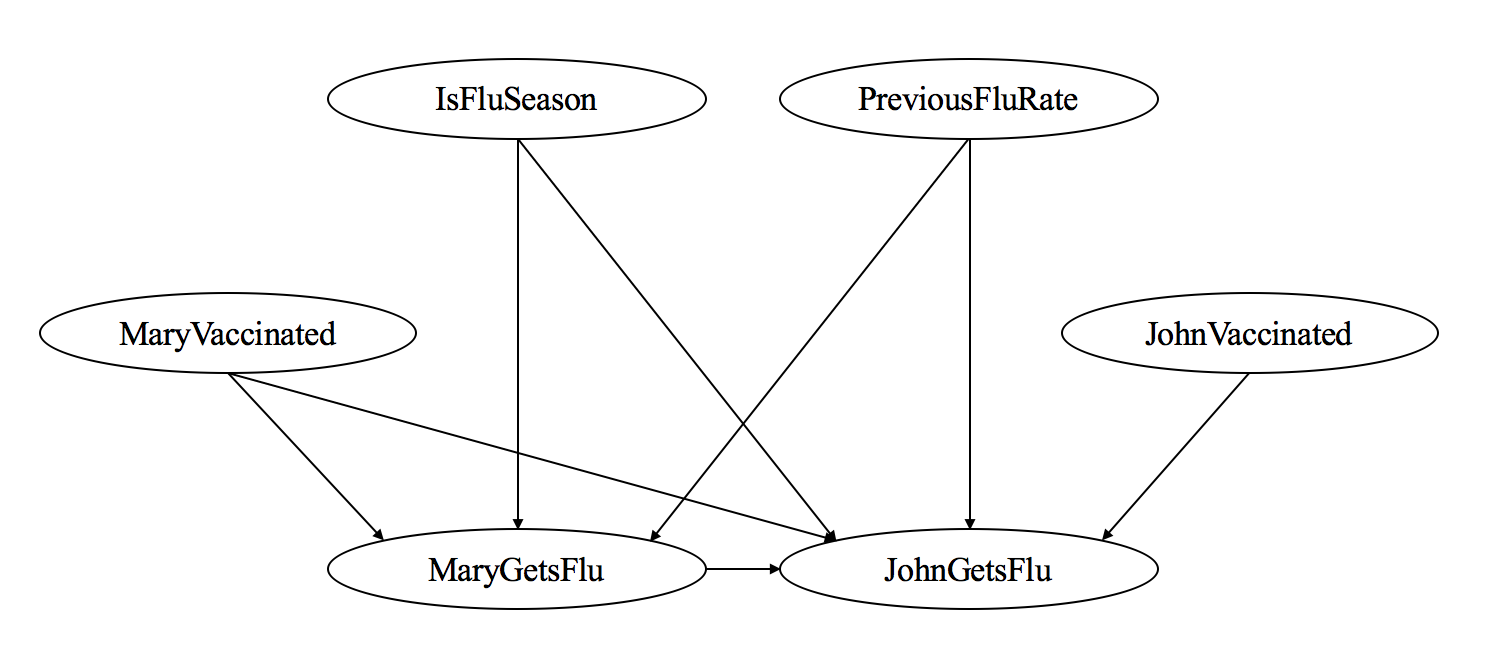
\includegraphics[scale=0.6]{i-map}
\end{center}

\noindent
\large \textbf{2.1.2 Analytical Question [6 points]}\\
\textbf{Ans:}\\
In 2.1.1, we had applied the "Algorithm 3.2 Procedure to build a minimal I-map given an ordering" to find the minimal I-map. For this problem, since a node $E$ is eliminated from the original graph, the new independence set is a subset of the original independence set. For each independence rule that involves node $E$, we view the node $E$ as an unobserved node. For the ordering of variables $\mathcal{X}$, we can still keep it the same except that we take the node $E$ out of the order. Then we can apply the algorithm 3.2 again on the new graph using the original independence set while keeping the node $E$ unobserved to find the minimal I-map.\\

\newpage
\noindent \Large \textbf{2.2 Network Queries [16 points]}\\
\large \textbf{2.2.1. Analytical Questions}\\
\large 1. [8 points]\\
\textbf{Proof:}
Let's prove it by contradiction. Assume altering $Z$'s CPD cannot affect $P(X|\mathbf{Y})$, then there is no active trail from $Z$ to $X$ given $\mathbf{Y}$, i.e., $Z \bot X | \mathbf{Y}$. Since $\hat{Z}$ is a parent of $Z$, so $\hat{Z} \bot X | \mathbf{Y}$, i.e., there is no active trail from $\hat{Z}$ to $X$ given $\mathbf{Y}$, which contradicts the condition of the statement. So the assumption doesn't hold and the statement is true. $\square$\\
\\
2. [8 points]\\
\textbf{Proof:}
Let's prove it by contradiction. Assume altering $Z$'s CPD can affect $P(X|\mathbf{Y})$, then there is an active trail from $Z$ to $X$ given $\mathbf{Y}$. Since $\hat{Z}$ is a parent of $Z$, we can find an active trail from $\hat{Z}$ to $X$ given $\mathbf{Y}$ by going through $\hat{Z}\rightarrow Z$ then going through the active trail from $Z$ to $X$ given $\mathbf{Y}$. However, this contradicts the condition of the statement, so the assumption is false and the statement is true. $\square$\\
\\
\noindent \Large \textbf{2.3 Variable Elimination [12 points]}\\
\large 1. [8 points]\\
a.
\begin{center}
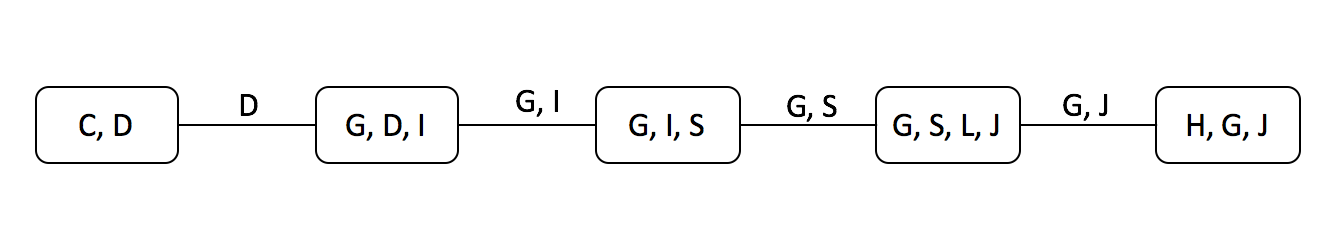
\includegraphics[scale=0.75]{a}
\end{center}

A clique tree is valid if it satisfies the family preservation property and the running intersection property. For problem (a), the clique tree satisfies the preservation property because each factor $\phi$ is associated with a cluster $C_i$ such that Scope[$\phi$]$\subseteq C_i$. And each edge between a pair of clusters $C_i$ and $C_j$ is associated with a sepset (separation set) $S_{i,j} \subseteq C_i \cap C_j$. This clique also satisfied the running intersection property because for any variable $X$ such that $X \in C_i$ and $X \in C_j$, $X$ is also in every cluster in the path between $C_i$ and $C_j$. So this clique tree is valid.\\
\\
\noindent
b.
\begin{center}
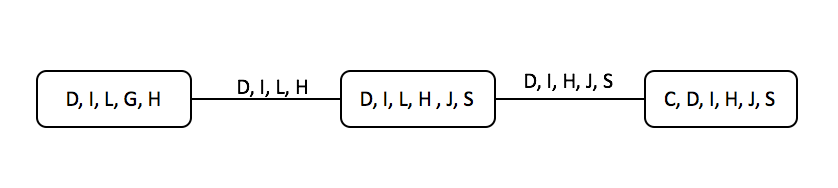
\includegraphics[scale=1]{b}
\end{center}

It is easy to show that this clique tree in problem (b) also satisfies the family preservation property and the running intersection property so it's valid.\\
\\
\noindent
\large 2. [4 points]\\
\textbf{Solution:}\\
$P(G,H,J) = P(H|G,J)\sum_{S,C} \sum_{L} P(J|L,S)P(L|G) \sum_{D} P(D|C)P(C) \cdot $ \\
$ \sum_I P(I)P(G|D,I)P(S|I)$

\end{document}